\documentclass[12pt]{article}
\usepackage[english]{babel}
\usepackage[utf8]{inputenc}
\usepackage{amsmath}
\usepackage{graphicx}
\graphicspath{{Images/}}
\usepackage[colorinlistoftodos]{todonotes}
\usepackage{hyperref}
%\usepackage{apple_emoji}
\usepackage{tikz}
\usepackage{subcaption}

\usepackage{parskip}
\setlength{\parindent}{1cm}
\usepackage{indentfirst}

\usepackage{enumitem}
\setitemize{noitemsep,topsep=0pt,parsep=0pt,partopsep=0pt}

\begin{document}
\begin{titlepage}
\newcommand{\HRule}{\rule{\linewidth}{0.1mm}} 
\center % Center everything on the page
 
%---------------------------------------------------------------------------------
%	HEADING SECTIONS (Enter the Homework/assignment No., only)
%---------------------------------------------------------------------------------
\textsc{\Large Linux/GNU}\\[0.3cm] % heading course Number
\textsc{\Large évaluation des avantages et des inconvénients de Yocto par rapport à Buildroot }\\[0.3cm] % heading course name

%---------------------------------------------------------------------------------
%	TITLE SECTION (Replace 'TITLE' with the Homework/assignment Name/title)
%---------------------------------------------------------------------------------

\HRule \\[0.4cm]
{ \huge \bfseries YOCTO}\\[0.1cm] % Title of your Homework/assignment
\HRule \\[1.5cm]
 
%---------------------------------------------------------------------------------
%	AUTHOR SECTION (EDIT THE NAME and T.NO., only)
%---------------------------------------------------------------------------------

\begin{minipage}{0.4\textwidth}
\begin{flushleft} \large
Colin \textsc{Baumgard}\\  % Enter Your name and T.No.
\end{flushleft}

\end{minipage}
\begin{minipage}{0.4\textwidth}
    \begin{flushleft} \large
        Paul-Antoine \textsc{Le Tolguenec}\\  % Enter Your name and T.No.
        \end{flushleft}

      
\end{minipage}\\[1cm]
{\large \today}\\[1cm] % Date, change the \today to a set date if you want to be precise

\includegraphics{ENSTA1246-524.png}% \\[0.5cm] % 
\vfill % Fill the rest of the page with white-space

\end{titlepage}
\include{GradingRubric}
\tableofcontents          % Required
\listoffigures
\listoftables
\newpage


% Chapters including
\section{Introduction}
\paragraph{}
ecris ici

\textbf{Repo GitHub}

\url{https://github.com/Paul-antoineLeTolguenec/Linux-GNU.git}

\newpage


\section{De Buildroot à Yocto}

\subsection{Buildroot}
\paragraph{}
Buildroot est un outil qui simplifie et automatise le processus de construction d'un système Linux complet pour un système embarqué, 
en utilisant la compilation croisée.

Pour y parvenir, Buildroot est capable de générer une toolchain, un RFS (root file system),
 un kernel Linux et un bootloader pour la cible. Buildroot peut être utilisé pour toute combinaison de ces options, 
 indépendamment (vous pouvez par exemple utiliser une chaîne de compilation croisée existante, 
 et ne construire que votre système de fichiers racine avec Buildroot). Ce qui permet de simplifier le processus en laissant tout de même beaucoup de liberté.

Les systèmes embarqués utilisent souvent des processeurs qui ne sont pas les processeurs x86 habituels que tout le monde est habitué à avoir dans son PC.
Créer son OS pour une architecture que peu de gens utilise s'avére très fastidieu.Il peut s'agir de processeurs PowerPC, de processeurs MIPS, de processeurs ARM, etc.
Buildroot rend le dévellopement del'OS adapté à ces processeurs très accessible.

\subsection{Yocto}
\paragraph{}
Yocto intègre des parties développées conjointement pour OpenEmbedded, notamment BitBake, OpenEmbedded-Core et d'autres métadonnées. 
Les éléments développés dans le cadre du projet, appelés "meta-yocto" et "meta-yocto-bsp", comprennent l'intégration des éclipses. 
Ensemble, ils améliorent les outils d'OpenEmbedded, cette plateforme de référence pour la construction de systèmes avancés embarqués dans les HW est connue 
sous le nom de Poky.

Pour développer des logiciels, nous avons besoin d'une chaîne d'outils (croisés) : les fichiers sources et les instructions sur la façon de les compiler. 
C'est suffisant pour une source. 
Pour plus de composants et de dépendances dans la compilation et le temps d'exécution, il faut augmenter la complexité et des étapes supplémentaires. 
Bitbake est un agent ayant la capacité d'interpréter et d'exécuter les recettes d'amélioration, il calcule la chaîne des tâches nécessaires pour développer l'objectif défini et exécuté. 


\input{Chapters/Building_OS_with_Yocto}
\section{Discussions et Conclusion}

\subsubsection{Yocto ou Buildroot, comment choisir ?}
\paragraph{}
Yocto est donc très adapté pour une image nécessitant une multitude de dépendances externes, pour un développement court et focalisé sur les fonctionnalités propres du produit, avec une gamme de produits proposant des fonctionnalités légèrement différentes. Yocto permet de factoriser le développement et de rendre modulable l'OS embarqué.  Buildroot est, quant à lui, plus adapté à des projets plus modestes, où la mise à jour est moins fréquente. Buildroot crée des OS statiques, adaptés aux outils plus bas niveau, peut être moins évolués, se focalisants sur la robustesse. Buildroot est également plus simple à prendre en main, ce qui est un atout non négligeable. Il sera en revanche moins adapté au travail en groupe. 


\begin{figure}[ht!] 
\begin{center}
    

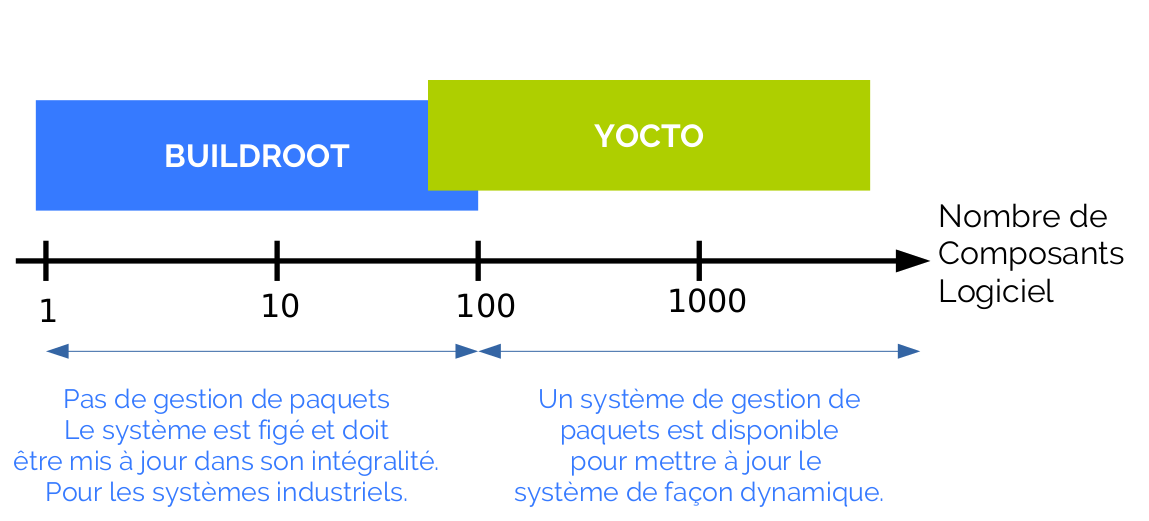
\includegraphics[width=13cm]{Images/yocto comp log.png} % Figure image 

\caption{crédit: Yocto project} % Figure caption 

\end{center}
\label{Project Yocto} % Label for referencing with \ref{bear} 
\end{figure}

On peut donc résumer : 
Le projet
\begin{itemize}

\item comporte une gamme de produit - Yocto facilitera la factorisation du développement
\item comporte de nombreux modules externe - Yocto
\item repose sur des ajouts de fonctionnalité fréquentes - Yocto
\item est un système figé, un code métier peu évolutif et peu de composants externe - Buildroot fera très bien l'affaire
\end{itemize}

Tout ce que peut faire Buildroot, Yocto en est également capable. Le passage de Buildroot à Yocto est pertinent si le projet est important, qu'il doit être porté sur différentes plateformes et qu'il nécessite de nombreuses composantes de la communauté. Si la composante centrale du projet n'est pas logiciel, que tout repose sur le code métier, avec un cycle de développement long, Buildroot est adapté et une évolution n'est pas forcément pertinente.


\bibliographystyle{unsrt}
\bibliography{./Chapters/Bibliographie}

\end{document}
